\documentclass{beamer} 
\usepackage{amsmath,amsthm}
\usepackage{graphicx,microtype,parskip}
\usepackage{caption,subcaption,multirow}
\usepackage{attrib}

\frenchspacing

\usetheme{default}
\usecolortheme{whale}

\setbeamertemplate{navigation symbols}{}

\setbeamercolor{title}{fg=blue,bg=white}

\setbeamercolor{block title}{fg=white,bg=gray}
\setbeamercolor{block body}{fg=black,bg=lightgray}

\setbeamercolor{block title alerted}{fg=white,bg=darkgray}
\setbeamercolor{block body alerted}{fg=black,bg=lightgray}

\title{Death and taxa}
\subtitle{time-invariant differences in mammal species duration}
\author{Peter D Smits}
\institute{Committee on Evolutionary Biology}
\titlegraphic{
  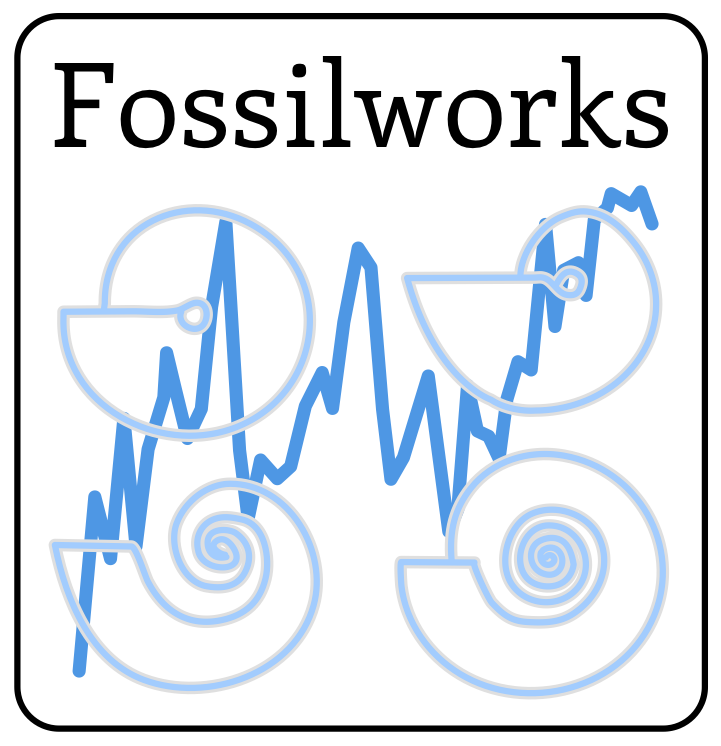
\includegraphics[width=1.75cm,height=1.75cm,keepaspectratio=true]{figure/fossilworks}
  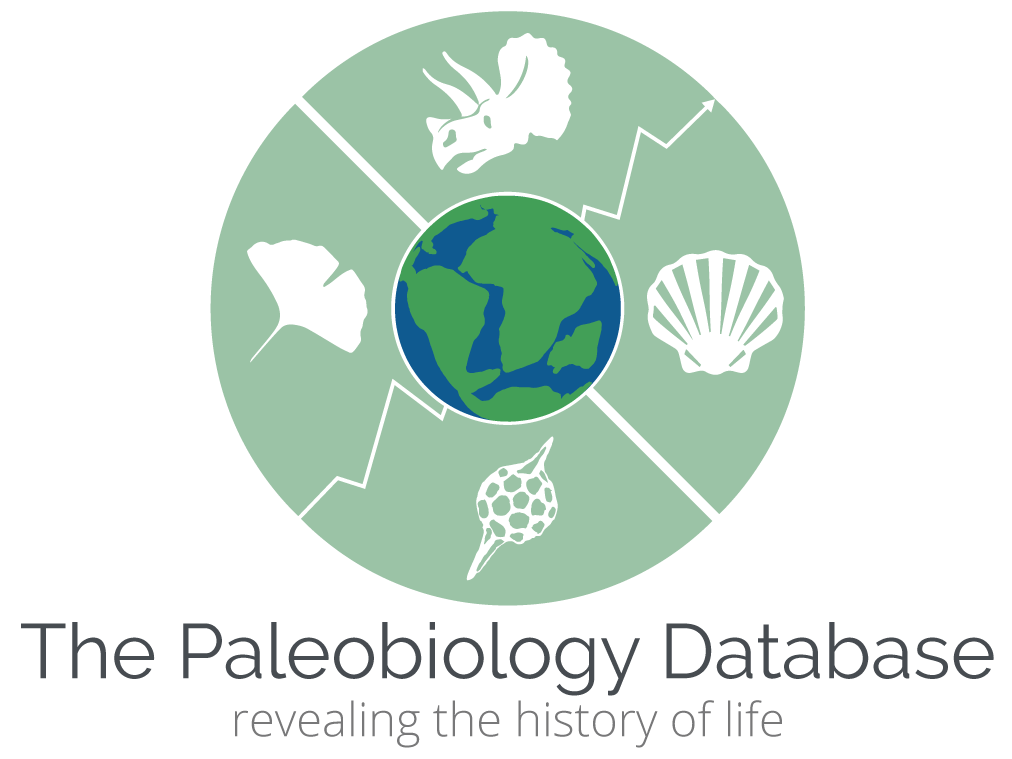
\includegraphics[width=2.5cm,height=2.5cm,keepaspectratio=true]{figure/paleodb}
  \hspace*{0.35\paperwidth}
  
\includegraphics[width=1.75cm,height=1.75cm,keepaspectratio=true]{figure/chicago}
}
\date{}

\begin{document}

\begin{frame}
  \titlepage
\end{frame}

\begin{frame}
  \frametitle{Acknowledgements}
\end{frame}

\begin{frame}
  \frametitle{Differences in species duration}

  \begin{block}{Framework}
    \begin{itemize}
      \item How do different species-level ecological traits relate to differences in species duration?
      \item How do time of origination and phylogenetic history contribute to differences in species duration?
      \item Does extinction risk vary with species duration?
    \end{itemize}
  \end{block}
\end{frame}

\begin{frame}
  \frametitle{Traits of interest}
\end{frame}

\begin{frame}
  \frametitle{Body size}

  Three hypotheses
\end{frame}

\begin{frame}
  \frametitle{Dietary category}

  carnivory, herbivory, insectivory, omnivory
\end{frame}

\begin{frame}
  \frametitle{Locomotor category}

  arboreal, ground dwelling, scansorial
\end{frame}

\begin{frame}
  \frametitle{Bayesian survival model}
\end{frame}

\begin{frame}
  \frametitle{Survival function}
\end{frame}

\begin{frame}
  \frametitle{Variance partitioning coefficients}
\end{frame}

\begin{frame}
  \frametitle{Current biodiversity crisis}
\end{frame}

\begin{frame}
  \frametitle{Concerns}
\end{frame}

\begin{frame}
  \frametitle{Conclusions}
\end{frame}

\appendix

\begin{frame}
  \frametitle{Posterior predictive checks: deviance residuals}
\end{frame}

\begin{frame}
  \frametitle{Posterior predictive checks: point check}
\end{frame}

\end{document}
